\documentclass[14pt]{article}
\usepackage[utf8]{inputenc}
\usepackage[russian]{babel}
\usepackage{graphicx}
%\usepackage{float}
\usepackage{floatrow}
\usepackage{caption}

\newfloatcommand{capbtabbox}{table}[][\FBwidth]
\newfloatcommand{capbfigbox}{figure}[][\FBwidth]

\begin{document}
\begin{titlepage}
	\begin{center}
		ФЕДЕРАЛЬНОЕ ГОСУДАРСТВЕННОЕ АВТОНОМНОЕ ОБРАЗОВАТЕЛЬНОЕ  \\
		УЧРЕЖДЕНИЕ \\
		ВЫСШЕГО ПРОФЕССИОНАЛЬНОГО ОБРАЗОВАНИЯ \\
		НАЦИОНАЛЬНЫЙ ИССЛЕДОВАТЕЛЬСКИЙ УНИВЕРСИТЕТ\\
		<<ВЫСШАЯ ШКОЛА ЭКОНОМИКИ>> \\
		МОСКОВСКИЙ ИНСТИТУТ ЭЛЕКТРОНИКИ И МАТЕМАТИКИ \\
		\vspace{5ex}
		Департамент Прикладной Математики
		\vspace{0.5ex}
		
	\end{center}
	
	\vspace{15ex}
	\begin{center}
		Колотев Сергей Васильевич\\
		\vspace{1ex}
		\textbf{Моделирование пространственных эволюционных игр}\\
		\vspace{5ex}
		Междисциплинарная курсовая работа \\
		студента группы МСУ161(образовательная программа\\
		<<Системы управления и обработки информации в инженерии>>)
		
	\end{center}	
	\vspace{15ex}
	\begin{flushright}
		\noindent
		Научный руководитель
		\\
		профессор, д. ф.-м. н.\\
		заведующий базовой\\
		кафедрой "ПИКСиС"\\
		ДПМ МИЭМ ВШЭ\\
		Щур Лев Николаевич
	\end{flushright}
	
	
	
	\begin{center}	
		\vfill
		Москва 2017
	\end{center}
\end{titlepage}

\tableofcontents

\newpage
\section{Введение}
\par Данная работа является продолжение бакалаврской выпускной квалификационной работы на тему <<Моделирование пространственных эволюционных игр>>. Исследования в текущей и бакалаврской работе основаны на результатах статьи Р.Мэй и М. Новака, опубликованной в 1992 о пространственной дилемме об эволюции. \par В ней за основу взята модель Дилеммы Узника, помещенная на квадратную решетку с периодическими граничными условиями. В стандартной Дилемме Узника двое игроков играют друг против друга, выбирая стратегии. Дефектор получает максимум очков(T), если играет против кооператора, а кооператор в данной ситуации получает минимум(S). Если дефектор играет против дефектора, оба получат одинаковое количество очков(P) в промежутке между максимальным и минимальным. В случае если кооператор играет против кооператора, то здесь оба игрока получают количество очков(R) меньше максимума, но больше очков, чем в ситуации, когда дефектор играет против дефектора. Каждый игрок знает исход предыдущей игры и делает выбор на основе этой информации. В этом заключается стандартная Дилемма Узника.
\par Р.Мэй и М. Новак решили расположить игроков на решетку с периодическими граничными условиями и зафиксировать все очки, получаемые игроками, кроме максимального, которые получает дефектор за победу над кооператором. Таким образом модель Дилеммы Узника стала клеточным автоматом, в котором каждый игрок представляет собой ячейку со множеством состояний являющихся множеством стратегий. Ячейка или игрок могут быть кооператором или дефектором. Окрестность - это 8 соседей вокруг текущей ячейки. В начальном состоянии решетка заполняется случайным образом на 90\% кооператоров, а также задано правило перехода, которое определяет новое состояние ячейки или иными словами, определяет, какую стратегию выберет игрок на следующем этапе. Правило гласит, что в следующем поколении игрок возьмет стратегию того соседнего игрока, чей доход от игры со своими соседями будем максимальным. Каждый игрок играет с 8 соседями и сам с собой, поэтому в определении состояния ячейки принимают участие 25 клеток. Вся система переходит в новое состояние(поколение), когда каждый игрок сыграл со своими соседями и определил новую стратегию. Количество поколений является аналогом времени t. Количество очков, получаемых при игре кооператора против кооператора равно 1, дефектора против дефектора равно 0. Кооператор при игре с дефектором также получает 0 очков, в то время как дефектор получается максиматльное количество очков Т, что является параметром в данной модели. Такую модель описали Р.Мэй и М. Новак и, проведя на ней вычисления, пришли к интересным результатам. 
\par При симметричном начальном состоянии на решетке образуется <<динамический фрактал>> и <<эволюционирующие калейдоскопы>>. Также найдены устойчивые образования, которые называются <<glyder>>, <<grower>> и <<rotator>>.  На решетке могут существовать как кооператоры, так и дефекторы, это зависит от максимального дохода во время игры. При разных значениях параметра Т на решетке наблюдаются различные состояния, при Т<=1 на решетке вымирают все дефекторы, остаются только кооператоры, аналогично при Т>=2 остаются только дефекторы. Игроки, имеющие среди своих соседей игроков с такой же стратегией, образуют структуру под названием кластер. Следовательно, существуют два типа кластеров - из кооператоров и дефекторов. При параметре Т<1.8 растут только кластеры из кооператоров, иными словами, на решетке будет большинство игроков будут выбирать стратегию кооператора. Кластеры такого типа будут продолжать расти при Т<2. В случае Т>1.8 начинают расти кластеры из дефекторов. Кроме того, обнаружен фазовый переход в Т=1.8. Именно в промежутке 1.8<=T<=2 кластеры обоих типов могу расти и сталкиваться в процессе роста и в данной ситуации, было вычислено, что при t -> $inf$ концентрация кооператоров сходится к значения $12log2 - 8 = 0.31776617...$
\par В бакалаврской работе была воспроизведена данная модель с помощью языков программирования Python и C. Первый вариант производил вычисления достаточно долго на решетках размера 100х100 и более, поэтому было принято решение переписать алгоритм, используя язык С. Помимо того, что компилируемый код выполняется гораздо быстрее интерпретируемого, алгоритм был дополнен инструментами параллельного программирования OpenMP. Эта технология включается в себя набор директив и команд для процессора, позволяющих распределить одинаковые вычисления между нитями процессами. OpenMP достаточно прост для внедрения и не требует серьёзных изменений в программе.
\par Для применения OpenMP необходимо было узнать, какой участок кода нужно распределять между нитями процессора. Параллельно могут вычисляться те части кода, где данные между собой не зависят друг от друга, иначе можно получить неверные результаты. Таким образом применить OpenMP для расчета каждого поколения является неправильным решением, так как очередное состояние решетки строится исходя из предыдущего состояния. Однако, оказалось, что можно считать параллельно строки решетки. Иными словами, распределить между нитями процессора строки матрицы, чтобы каждая нить определяла новое состояние определенной строки решетки в следующем поколении.
\par Благодаря OpenMP, удалось значительно ускорить время выполнения программы, также стало возможным производить расчеты на решетках размером свыше 300х300. Из-за того, что открытие и закрытие параллельного участка кода требует большого числа операций, выполнение программы с использованием параллельного программирования на решетка размеров менее 100х100 использовать не следует. 
\par Текущих инструментов было достаточно лишь для общей картины. С их помощью было вычислено, что точка фазового перехода является T=1.8 с точностью $10^{-5}$. Но чтобы понять, что происходит с объектами на решетке, необходимо было выявить эти объекты. Была поставлена задача выделить на решетке кластеры обоих типов, применив алгоритм Хошена-Копельмана(HK-76). Данный алгоритм позволяет за один проход выделить кластеры на решетке. После его применения можно узнать размеры кластеров, а также к какому из них принадлежит та или иная ячейка. Благодаря этому алгоритму было выяснено, что средний размер наибольшего кластера кооператоров при параметре Т=1.79999(вблизи точки фазового перехода) в текущем состоянии занимает приблизительно 70\% размера решетки, при стремлении ее размера к бесконечности. 
\section{Подсчет периметра и границы кластера}
\par В этой главе будут рассмотрены несколько алгоритмов поиска границы протекающих кластеров. Для начала стоит дать определение протекающему кластеру. Данное понятие пришло из теории перколяции(с англ. - протекание, просачивание), которая изучает связные структуры. Область применения теории перколяции на сегодняшний день довольно обширная, начиная с маршрутизации в сети интернет и заканчивая распространением лесных пожаров. Также она нашла свое применение в медицине, физике и химии. Перколяция возникает, когда элементы структуры расположены таким образом, что можно совершить переход по ее элементам с одной стороны на другую. Таким образом, протекающим кластером является такой кластер, по элементам которого можно пройти от верхней границы решетки к нижней или наоборот. Аналогично можно рассматривать и переход слева направо и в обратную сторону, и так как они схожи, то будет рассматриваться первый вариант.
\par Поиск протекающего кластера осуществляется следующим образом. Каждый кластер имеет свой номер, в первой строке решетки берется первый помеченный(принадлежащий какому-либо кластер) элемент, и ищется другой, входящий в состав этого же кластера, но уже в последней строке решетки. Конечно, может быть случай, когда у нас кластер не является протекающим, хотя его элементы присутствуют как в первой, так и в последней строке. В таком случае для поиска границы, можно убрать периодичность сверху и снизу, тогда такие кластеры не будут считаться за один. Но для общей статистики по количеству и размеров кластеров, периодичность по верхней и нижней границе необходимо учитывать.
\par Для определения границы протекающего кластера нужно перейти от обычной решетки к дуальной. Если в двумерную плоскую решетку внедрить новую путем расположения в  центрах ячеек дополнительных узлов и соединить эти узлы между собой, то полученная система будет называться дуальной решеткой. 
\par Дадим определение границы протекающего кластера. Данную величину можно задать несколькими способами. Один из них следующий: граница - это множество элементов протекающего кластера, среди соседей которых есть хотя бы один элемент, принадлежащий кластеру другого типа, соответственно величина границы - это мощность этого множества, т.е. количество этих элементов.  Но существуют случаи, когда у протекающего кластера нет границы, например, когда есть один большой кластер одного типа, в котором находятся несколько небольших кластеров другого. В этом случае что является границей такого кластера сказать сложно. Поэтому, чтобы не возникало таких случаев при расчете длинны границы, необходимо условие, что на решетке в текущем состоянии есть протекающие кластеры обоих типов. В такой ситуации можно утверждать, что у протекающего кластера интересующего нас типа точно есть граница.
\par Теперь можно описать алгоритм подсчета размера границы. На текущем шаге известны номера протекающих кластеров. Для того, чтобы проще было обойти его границу, ее можно пометить. Для того, чтобы понять, какой элемент нужно пометить, необходимо посмотреть каждый на наличие среди соседей элемент кластера другого типа. После пометки всех граничных элементов, нужно взять любой помеченный элемент в первой строке и переходить к соседнему помеченному. Первыми проверяем, есть ли помеченные соседние элементы снизу, далее сбоку, и затем уже сверху(если текущий элемент не в первой строке). Нужен счетчик переходов, который увеличивается на единицу, когда происходит переход. Величина такого счетчика как раз и будет являться величиной границы. Чтобы не попасть в цикл, убираем метку после перехода, чтобы не рассматривать элемент как граничный. Также следует учитывать периодичные граничные условия.
\par Этот алгоритм имеет серьезный недостаток. Например, если зайти в тупик, то он никогда не завершится, поэтому приходится либо начинать обход границы с другого элемента первой строки, либо возвращать величину границы равную нулю. Данная проблема решается путем изменения алгоритма на рекурсивный. При переходе необходимо знать следующие характеристики - метку элемента, номера протекающих кластеров обоих типов, текущую позицию и текущую длину. Алгоритм останавливается, когда достигнута последняя строка. Придя в тупик, происходит откат на последний элемент, у которого среди соседей было несколько помеченных элементов, и так как при переходе метка убирается, то на этот раз переход будет на новый элемент. Также при возврате длину границы не нужно пересчитывать, но необходимо иметь флаг, сигнализирующий о виде возврата, ведь возврат в рекурсии осуществляется и при окончании работы алгоритма. Но и рекурсия всех проблем не решает. В текущей реализации не решены проблемы выбора границы, ведь алгоритм проходит по какой-то границе, а не минимальной. К тому же все направления соседей равнозначны, и какой элемент проверять на наличие метки первым также является проблемой. Кроме того, при обходе по помеченным элементам иногда угловые элементы учитываются, а иногда нет, хотя они тоже составляют часть границы.
\par Исходя из наличия множества недостатков, было принято решение рассмотреть полную границу протекающего кластера. Иными словами его периметр. Для этого не требуется, чтобы на в текущем состоянии были протекающие кластеры обоих типов, также не нужно помечать границу. Для вычисления периметра необходимо знать лишь номер протекающего кластера. К тому же периметр считается не как количество элементов, которые являются граничными, а как число связей между ними и элементами кластера другого типа. Такая величина является поверхностным натяжением системы, что характеризует раздел двух фаз. Другими словами, поверхностное натяжение пропорционально свободной энергии единицы площади поверхностного слоя. Алгоритм расчета периметра протекающего кластера довольно простой. Необходимо поэлементно рассмотреть протекающий кластер и посчитать сколько встречается элементов кластера другого типа. Количество таких элементов равно количеству связей на дуальной решетке.
\section{Анализ результатов}
\par В данной главе приведены результаты расчетов границ и периметров протекающих кластеров в зависимости от параметра Т вблизи фазового перехода, слева и справа.
\\

\par Были произведены вычисления одной границы протекающего кластера кооператоров, алгоритм которого был описан в предыдущей главе. В Таб.1 представлены данные о длине границы(SIZE) на разных размерах решетки(L). В последнем столбце(SD) указано стандартное отклонение величины границы. 

\begin{figure}[H]
	\begin{floatrow}
		\capbfigbox{%
			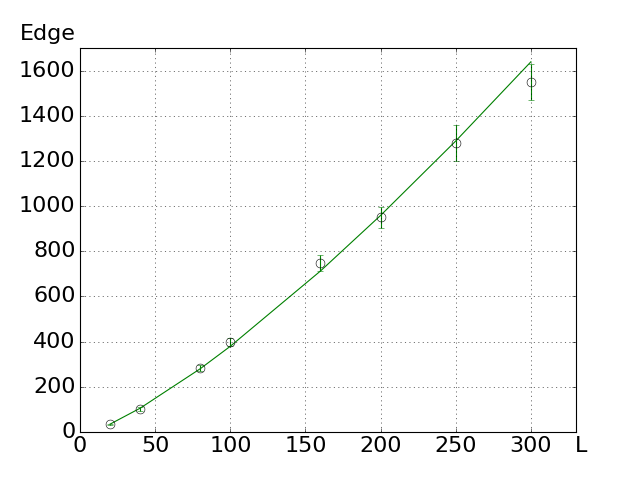
\includegraphics[scale=0.4]{edge.png}
			\label{fig:edge}
		}{\caption{T=1.799999}}
	
		\capbtabbox{ 				
			\begin{tabular}[H]{|c|c|c|}
				\hline 
				L& SIZE& SD\\
				\hline 
				20& 35.2463399& 7.0424445\\
				\hline 
				40& 101.6865767& 16.0999028\\
				\hline 
				80& 285.2107208& 61.2270698\\
				\hline 
				100& 397.3557487& 84.6384228\\
				\hline 
				160& 748.1331192& 166.3291768\\
				\hline 
				200& 950.2522597& 228.5622371\\
				\hline 
				250& 1278.614018& 364.1477427\\
				\hline 
				300& 1548.5866635& 420.3067575\\
				\hline
			\end{tabular}	
			 
		}{\caption{T=1.799999}}
	\end{floatrow}
\end{figure}


\begin{figure}[H]
	\begin{floatrow}
		\capbfigbox{%
			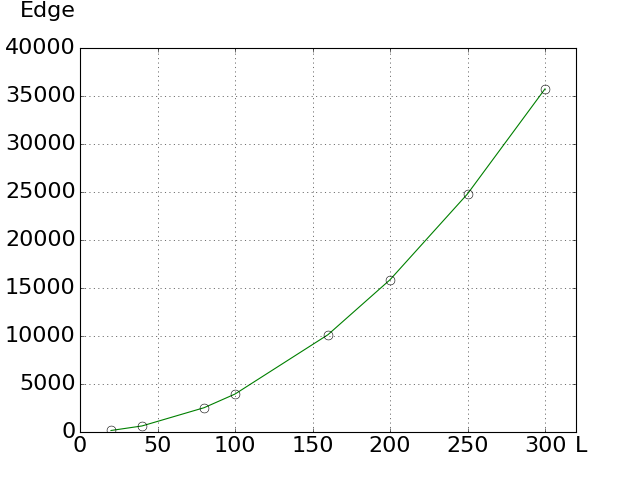
\includegraphics[scale=0.4]{t179999.png}
			\label{fig:179999}
		}{\caption{T=1.799999}}
		\capbtabbox{%
			\begin{tabular}[H]{|c|c|c|}
				\hline 
				L& SIZE& SD\\
				\hline 
				20& 157.363933& 0.9588096\\
				\hline 
				40& 627.7152318& 2.4366698\\
				\hline 
				80& 2527.0690522& 5.2422666\\
				\hline 
				100& 3952.660201& 5.4635683\\
				\hline 
				160& 10141.177825& 10.9722955\\
				\hline 
				200& 15873.1174448& 12.7376727\\
				\hline 
				250& 24780.7929112& 16.6012481\\
				\hline 
				300& 35744.8596091& 20.3251594\\
				\hline
			\end{tabular}	
			\label{tab:1.799999} 
		}{\caption{T=1.799999}}
	\end{floatrow}
\end{figure}

\begin{figure}[H]
	\begin{floatrow}
		\capbfigbox{%
			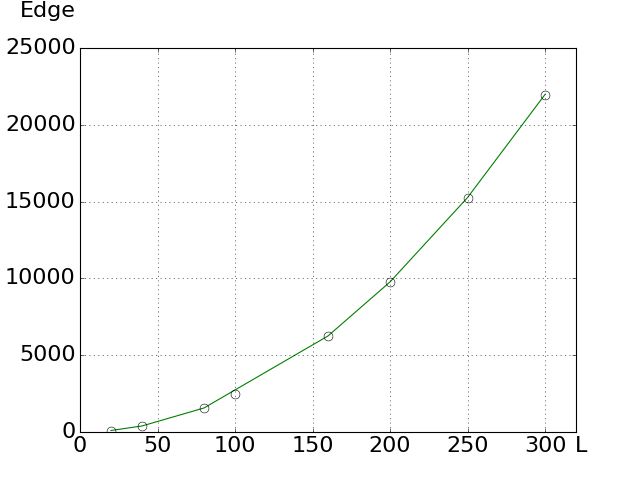
\includegraphics[scale=0.4]{t185.png}
			\label{fig:1.85}
		}{\caption{T=1.85}}
		\capbtabbox{%
			\begin{tabular}[H]{|c|c|c|}
				\hline 
				L& SIZE& SD\\
				\hline 
				20& 38.4244482& 4.7300971\\
				\hline 
				40& 391.7066584& 0.0361383\\
				\hline 
				80& 1564.3151184& 0.0876022\\
				\hline 
				100& 2443.3837938& 0.1482743\\
				\hline 
				160& 6252.5685688& 0.1674222\\
				\hline 
				200& 9767.1632024& 0.255711\\
				\hline 
				250& 15260.4871784& 0.2750390\\
				\hline 
				300& 21972.6163012& 0.3701978\\
				\hline
			\end{tabular}	
			\label{tab:1.85} 
		}{\caption{T=1.85}}
	\end{floatrow}
\end{figure}
	
\begin{figure}[H]
	\begin{floatrow}
		\capbfigbox{%
			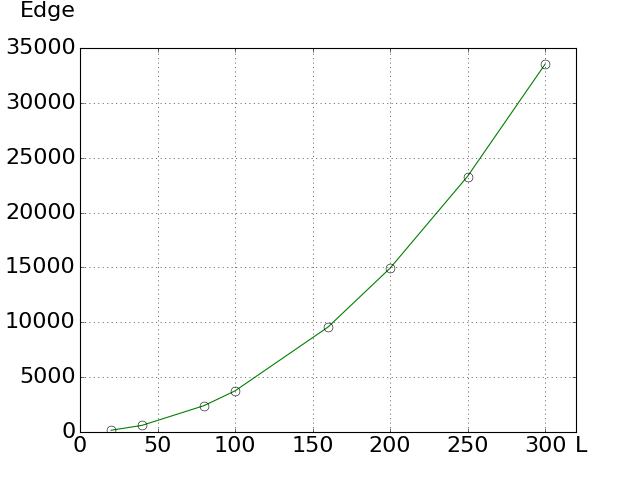
\includegraphics[scale=0.4]{t175.png}
			\label{fig:1.75}
		}{\caption{T=1.75}}
	\capbtabbox{%
	\begin{tabular}{|c|c|c|}
		\hline 
		L& SIZE& SD\\
		\hline 
		20& 155.3604996& 1.7692564\\ 
		\hline 
		40& 604.1202568& 2.9686895\\ 
		\hline 
		80& 2400.694044& 6.5851788\\ 
		\hline 
		100& 3755.3912588& 7.4496632\\ 
		\hline 
		160& 9548.8415264& 11.6337259\\ 
		\hline 
		200& 14939.733194& 16.6682224\\ 
		\hline 
		250& 23269.6086632& 18.135744\\ 
		\hline 
		300& 33537.6329936& 24.8820207\\  
		\hline 
	\end{tabular}
	\label{tab:175} 
}{\caption{T=1.75}}
	
	\end{floatrow}
\end{figure}
\section{Заключение}
\par Полученный результаты являются неожиданными и интересными и требуют дальнейшего изучения. Также необходимо доработать и усовершенствовать алгоритм расчета одной границы протекающего кластера. А именно находить минимальную границу и понять, как она меняется с ростом системы.\\

\section{Список литературы}
\end{document}